% !TeX program = pdflatex
% !TeX encoding = UTF-8
\ifdefined\pdfminorversion
\pdfminorversion=7
\fi
\documentclass[runningheads]{llncs}

\usepackage{graphicx}
\usepackage{placeins}
\usepackage{float}
\usepackage{booktabs}
\usepackage{multirow}
\usepackage{array}
\usepackage{amsmath}
\usepackage{amssymb}
\usepackage{xcolor}
\usepackage{tikz}
\usetikzlibrary{positioning,arrows.meta,fit,calc}
\usepackage{url}
\usepackage[hidelinks]{hyperref}
\usepackage{marvosym}

\newcommand{\sys}{XJDX\_001}
\newcommand{\method}{DualFaith}
\newcommand{\mf}{Macro-F1}
\newcommand{\pem}{PEM}
\newcommand{\joint}{Joint@3}
\newcommand{\lab}[1]{\textsf{\small #1}}
\newcommand{\best}[1]{#1}
\definecolor{steel}{RGB}{74,111,165}
\definecolor{brick}{RGB}{193,67,47}
\definecolor{teal}{RGB}{42,157,143}
\definecolor{amber}{RGB}{184,124,0}
\raggedbottom
\emergencystretch=2em
\setlength{\textfloatsep}{8pt plus 2pt minus 2pt}
\setlength{\floatsep}{8pt plus 2pt minus 2pt}
\setlength{\intextsep}{8pt plus 2pt minus 2pt}
\setlength{\abovecaptionskip}{4pt}
\setlength{\belowcaptionskip}{0pt}
\let\oldthebibliography\thebibliography
\let\endoldthebibliography\endthebibliography
\renewenvironment{thebibliography}[1]{%
  \oldthebibliography{#1}%
  \fontsize{8}{8.2}\selectfont
  \setlength{\itemsep}{0pt}%
  \setlength{\parskip}{0pt}%
  \setlength{\parsep}{0pt}%
}{\endoldthebibliography}

\begin{document}

\title{\texorpdfstring{\method{} at NLPCC-2026 Task 10:\\
Faithfulness Verification for Scientific Reports against Experimental Results and Citation Evidence}{DualFaith at NLPCC-2026 Task 10: Faithfulness Verification for Scientific Reports against Experimental Results and Citation Evidence}}
\titlerunning{Faithfulness Verification for Scientific Reports}

\author{Wenbiao Zhao\inst{1}\thanks{Wenbiao Zhao and Longkun Shi contributed equally to this work.} \and
Longkun Shi\inst{1}\textsuperscript{$\star$} \and
Zicheng Zuo\inst{1,2,3} \and
Turdi Tohti\inst{1,2,3}\textsuperscript{\Letter}}
\authorrunning{W. Zhao et al.}
\institute{
School of Computer Science and Technology, Xinjiang University, Urumqi 830017, China
\and
Joint International Research Laboratory of Silk Road Multilingual Cognitive Computing, Urumqi 830017, China
\and
Xinjiang Key Laboratory of Signal Detection and Processing, Urumqi 830017, China\\
\email{turdy@xju.edu.cn}}

\maketitle

\begin{abstract}
NLPCC-2026 Shared Task 10 addresses faithfulness risks in AI-assisted scientific reporting, where fluent text must also be supported by experimental results or cited papers. The two tracks expose complementary error structures. Track~1 is limited mainly by minority-class recall and paragraph exact match, whereas Track~2 is challenged by the coupling between retrieval and label prediction under domain shift. Track~1 assigns one of five faithfulness labels to each sentence in a scientific results paragraph using figure or table evidence. Our Track~1 system fine-tunes Qwen3-VL-8B-Instruct with LoRA, a softmin-PEM paragraph-bottleneck loss, minority-class oversampling, and a recall-additive union ensemble. It scores 50.61 in Phase~1 with the highest \mf{} of 57.54 among all teams, and ranks second among 11 teams with a final score of 68.79, only 0.11 behind first place. Track~2 assigns one of four citation-support labels to an atomic claim using the full text of the cited paper and returns the supporting paragraphs. Our Track~2 system freezes the evidence list produced by BM25 and four fused rerankers, then stacks a DeBERTa evidence reader, a claim-only classifier, an external NLI posterior, and a logistic-regression meta-classifier. It scores 86.27 and ranks first among 15 teams.
\keywords{Scientific report faithfulness \and Multimodal claim verification \and Citation faithfulness \and Domain shift \and Ensemble learning}
\end{abstract}

\section{Introduction}

AI-assisted writing is increasingly used to draft scientific reports, summarize experiments, and describe related work, but every generated scientific statement must satisfy one basic requirement: relevant evidence must support it. A results paragraph may report values from a figure correctly, but it may also assert an unsupported mechanism, refer to the wrong dataset, or extend a local finding beyond its valid scope. Likewise, a related-work statement may include a citation even when the cited paper does not support it. Faithfulness in scientific reporting is therefore not a single fact-checking problem, but a set of fine-grained verification tasks defined over different evidence forms.

NLPCC-2026 Shared Task 10, Reliability of AI-Assisted Scientific Reporting~\cite{nlpcc2026task10}, divides this problem into two complementary tracks. Track~1 focuses on experimental evidence. Given a multi-sentence scientific claim and corresponding figures or tables, a system assigns a faithfulness label to each sentence. Track~2 focuses on citation evidence. Given an atomic scientific claim and the paragraphs of its cited paper, a system determines the citation-support relation and returns the supporting paragraphs. Track~1 requires a vision-language model to read values, entities, and trends from rendered evidence, while Track~2 requires retrieval and full-document reading to distinguish \lab{Supported}, \lab{Overstate}, \lab{Topical Match}, and \lab{Irrelevant}. Both tracks use metrics that accumulate local errors. The Track~1 score combines sentence-level \mf{} with paragraph exact match, denoted by \pem{}. Missing a single minority-class sentence in a long paragraph makes the entire paragraph ineligible for \pem{}. The Track~2 \joint{} metric requires both the correct label and a retrieved gold paragraph, so either a retrieval error or a classification error causes the record to fail. This coupling prevents a system from optimizing one module in isolation and instead requires a balance among recall, precision, evidence retrieval, and label robustness.

We refer to the combined approach as \method{}(original name \sys{}). For Track~1, we found that the recall increases as the system recovers more minority-class sentences, while suppression heuristics reduce performance. We therefore fine-tune Qwen3-VL-8B-Instruct~\cite{qwen3vl2025} with LoRA~\cite{hu2021lora} for sentence-level multimodal classification and use a union ensemble to accumulate minority-class recall across members. For Track~2, the training data and the two test phases differ sharply in domain. Phase~1 is dominated by physics and materials science, while Phase~2 returns to a computer-science-dominated distribution. We therefore freeze a strong evidence list early and concentrate subsequent improvements on label-side signals that are less sensitive to domain shift.

This paper makes four contributions.
\begin{enumerate}
\setlength{\itemsep}{0pt}
\setlength{\parsep}{0pt}
\item It formulates and analyzes faithfulness verification over experimental figures and the full text of cited papers.
\item For Track~1, it develops a sentence-level vision-language approach with long-tail resampling, density-matched augmentation, and a two-stage recall-additive union.
\item For Track~2, it introduces a citation-support approach that combines evidence fusion with domain-robust label stacking from an evidence reader, a claim-only classifier, and an external NLI posterior.
\item It reports official results and negative findings that show how metric coupling, development-set shift, and ensemble selection shape shared-task performance.
\end{enumerate}

\section{Related Work}

\subsection{Multimodal Verification of Experimental Results}
Track~1 concerns multimodal claim verification against figures and tables. Captions often omit the values, entity names, legends, and relative trends that determine whether a claim is faithful, so a model must read the rendered evidence directly. The Qwen-VL family provides strong backbones for joint image and text understanding~\cite{qwen3vl2025}, while parameter-efficient methods such as LoRA enable task-specific adaptation under limited computational resources~\cite{hu2021lora}. Our Track~1 system follows this direction, but its central finding concerns the interaction among minority-class recall, the paragraph-level metric, and priors induced by the training distribution rather than an isolated gain from model scale.

\subsection{Parameter-Efficient Tuning and Multimodal Ensembles}
Vision-language models for scientific chart understanding must process images, captions, and claim text jointly. Parameter-efficient tuning reduces memory and training costs by updating only low-rank adapters~\cite{hu2021lora}, which is well suited to rapid adaptation in shared tasks. Multiple members trained with different sampling schemes, input formats, and random seeds can make complementary errors. In Track~1, this complementarity appears primarily as accumulated minority-class recall rather than confidence smoothing through simple probability averaging.

\subsection{Citation-Level Scientific Claim Verification}
Scientific claim verification is commonly formulated as evidence retrieval followed by entailment classification. FEVER defines open-domain verification as retrieving evidence from Wikipedia and predicting whether a claim is supported, refuted, or unverifiable~\cite{thorne2018fever}. SciFact transfers this setting to scientific abstracts and expert-written claims~\cite{wadden2020scifact}, while MultiVerS jointly models labels and rationales with a long-document encoder~\cite{wadden2022multivers}. Citation-level support is also closely related to attribution and hallucination detection in generated text~\cite{ji2023hallucination,rashkin2023attribution}. Recent studies examine reference errors in scientific literature~\cite{zhang2025referr} and evaluate the faithfulness of citations in generated text~\cite{zhang2024citefaith}. Track~2 differs from these settings because it requires both a graded citation-support label and the relevant evidence paragraphs from the cited paper.

\subsection{Reranking, Ensembling, and Learning under Shift}
Multi-stage retrieval commonly uses BM25 for candidate recall and a cross-encoder or sequence-to-sequence model for reranking~\cite{robertson2009bm25,nogueira2020monot5}. The Track~2 evidence stage instead fuses four heterogeneous rerankers after per-record min--max normalization. Deep ensembles reduce variance by averaging models trained with different random seeds~\cite{lakshminarayanan2017ensembles}, whereas stacked generalization combines heterogeneous predictors through a learned second-level model~\cite{wolpert1992stacked}. Domain-adversarial training~\cite{ganin2016dann} and label-shift correction~\cite{lipton2018bbse} are standard responses to distribution shift, but neither improves Track~2. The stable signals are a claim-only classifier that does not read out-of-domain evidence and the entailment posterior of an external multi-task NLI model~\cite{sileo2024tasksource}.

\section{Task Definition and Data Analysis}

\subsection{Track 1: Sentence-Level Faithfulness against Figure and Table Evidence}
Each Track~1 instance is a record $r=(\mathcal{S}_r,\mathcal{E}_r)$. The claim paragraph $\mathcal{S}_r=(s_1,\ldots,s_n)$ is pre-segmented into sentences, and the evidence set $\mathcal{E}_r$ contains one or more figures or rendered tables with their captions. The system predicts one label $\hat{y}_i\in\mathcal{L}_1$ for each sentence. The label set contains \lab{Supported}, \lab{Unsupported Causal Mechanistic}, \lab{Unsupported Entity}, \lab{Scope Overgeneralization}, and \lab{Contradiction}.

\lab{Supported} indicates that the evidence fully supports the sentence. \lab{Unsupported Causal Mechanistic} marks a causal or mechanistic explanation that the evidence does not justify. \lab{Unsupported Entity} indicates a dataset, model, metric, or other entity absent from the evidence. \lab{Scope Overgeneralization} extends a local conclusion beyond its supported scope, while \lab{Contradiction} directly conflicts with a value or trend in the evidence. The Track~1 output is a label sequence of length $n$ aligned with the input sentences.

\subsection{Class Imbalance and Test-Density Shift in Track 1}
\label{sec:t1-data}
Table~\ref{tab:t1-labels} summarizes the Track~1 split sizes and label distribution, including primary-label counts, primary-label shares, any-of occurrences, and multi-label sentences. The key pattern is severe class imbalance, with all non-\lab{Supported} labels forming a small minority under the primary-label view.

\begin{table}[ht]
\centering
\caption{Track~1 split sizes and train--development label distribution. Count gives split size for dataset rows and primary-label count for label rows. Share is computed over 17,547 train--development sentences, and Any-of counts occurrences among all gold labels.}
\label{tab:t1-labels}
\small
\begin{tabular}{lrrr}
\toprule
Entry & Count & Share & Any-of\\
\midrule
Train--development records & 3,333 & -- & --\\
Train--development sentences & 17,547 & -- & --\\
Phase~1 test records & 586 & -- & --\\
Phase~1 test sentences & 5,096 & -- & --\\
\midrule
\lab{Supported} & 16,438 & 93.7\% & 16,438\\
\lab{Scope Overgeneralization} & 540 & 3.1\% & 605\\
\lab{Contradiction} & 216 & 1.2\% & 216\\
\lab{Unsupported Entity} & 213 & 1.2\% & 639\\
\lab{Unsupported Causal Mechanistic} & 140 & 0.8\% & 276\\
Minority classes total & 1,109 & 6.3\% & 1,736\\
Multi-label sentences & 527 & -- & --\\
\bottomrule
\end{tabular}
\end{table}

The training distribution also induces a critical prior. Among training paragraphs with at least six sentences, only 0.46\% contain two or more minority-class sentences, and only 8 of all 3,333 records satisfy this condition. A model can therefore learn an approximate rule of at most one minority-class sentence per paragraph. The Phase~1 test paragraphs are longer and much denser in minority classes, with approximately 84\% containing at least one minority-class sentence. Consequently, the all-\lab{Supported} baseline scores only 18.85 on the test set, compared with 43.2 on the train--development distribution. Under this test distribution, \pem{} is limited mainly by missed minority-class sentences rather than false positives.

\FloatBarrier

\subsection{Track 2: Citation Support against the Full Cited Paper}
Each Track~2 record pairs an atomic claim $c$ with a cited paper represented as paragraphs $D=\{P_1,\ldots,P_m\}$. The system outputs a label $y\in\mathcal{L}_2$, where $\mathcal{L}_2=\{\text{Supported},\text{Overstate},\text{Topical Match},\text{Irrelevant}\}$, and a ranked list $E$ of at most three paragraph identifiers. \lab{Supported} indicates that the cited paper supports the claim. \lab{Overstate} indicates that the claim is stronger or broader than the evidence. \lab{Topical Match} denotes topical relevance without support, and \lab{Irrelevant} indicates that the citation is unrelated to the claim.

\subsection{Domain Shift in Track 2}
The released Track~2 train--development set contains 2,162 records: 1,029 \lab{Supported}, 382 \lab{Irrelevant}, 376 \lab{Topical Match}, and 375 \lab{Overstate} instances. We hold out a stratified development set of 433 records and use the remainder for training. The Phase~1 test set contains 937 records, and the hidden Phase~2 test set contains 489.

Domain shift is the dominant factor in Track~2. Table~\ref{tab:t2-domains} reports coarse domain proportions estimated by a keyword classifier over claim text. The train--development set is dominated by computer science, AI, and machine learning, whereas Phase~1 is dominated by physics and materials science and Phase~2 returns to a computer-science-heavy distribution. Phase~1 is therefore an out-of-distribution evaluation, while Phase~2 is closer to an in-domain evaluation. The same system must remain stable under both validation regimes.

\begin{table}[t]
\centering
\caption{Domain composition of Track~2 claims estimated by a keyword classifier. Columns need not sum to 100\% because unclassified claims are omitted.}
\label{tab:t2-domains}
\small
\begin{tabular}{lccc}
\toprule
Domain & Train--development & Test Phase~1 & Test Phase~2\\
\midrule
Physics / Materials & 0.3\% & \best{64.8\%} & 0.6\%\\
CS / AI / ML & \best{49.3\%} & 2.2\% & \best{52.8\%}\\
Biology / Medicine & 3.0\% & 5.3\% & 1.8\%\\
Other / General & 47.5\% & 21.8\% & 44.8\%\\
\bottomrule
\end{tabular}
\end{table}

This shift has architectural and methodological consequences. An evidence reader is directly exposed to test documents from a new domain, while a classifier that reads only the claim inherits a weaker shift. In a topic-holdout probe, the claim-only classifier loses approximately 2 \mf{} points, compared with about 7 points for the evidence reader. Moreover, a development set sampled from the training distribution cannot reliably rank candidates for the physics-dominated Phase~1 test set. For both critical selection decisions that can be checked, the development set and the leaderboard favor opposite candidates.

\section{Method}
\FloatBarrier

\subsection{Track 1: Vision-Language Classification and Recall-Additive Ensembling}
Figure~\ref{fig:t1-system} illustrates the Track~1 formulation as sentence-conditioned multimodal classification. For each record, visual evidence, caption, and claim paragraph define a shared multimodal context, while each target sentence defines the prediction unit. A Qwen3-VL backbone is adapted with LoRA to estimate the faithfulness label of the target sentence. This parameter-efficient formulation preserves the pretrained visual-textual representation for numerical values, legends, and table structures while restricting task-specific learning to low-rank adapters.

\begin{figure}[t]
\centering
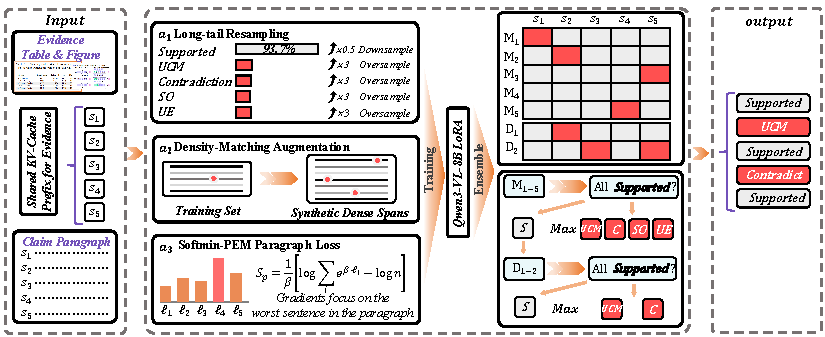
\includegraphics[width=\textwidth]{track1_figure.pdf}
\caption{Track~1 sentence-conditioned multimodal classifier. Qwen3-VL-8B is adapted with LoRA, long-tail resampling ($a_1$), density-matched augmentation ($a_2$), and the softmin-PEM surrogate ($a_3$); $M_{1\text{--}5}$ and $D_{1\text{--}2}$ form a recall-additive union over minority labels.}
\label{fig:t1-system}
\end{figure}

Training optimizes a per-sentence conditional likelihood under the shared record context. Each sample pairs the multimodal context with one target sentence and predicts its label. To reflect the paragraph-level exact-match constraint, the softmin-PEM objective augments token-level cross-entropy with a paragraph surrogate that assigns larger weight to the sentence most likely to invalidate the record. Section~\ref{sec:t1-sensitivity} compares this objective with plain cross-entropy, denoted by plain-CE, under controlled data conditions. Class imbalance is handled by minority-class oversampling and \lab{Supported} downsampling. To counter the training prior of at most one minority-class sentence per paragraph described in Section~\ref{sec:t1-data}, we construct density-matched examples by inserting real minority-class sentences into long paragraphs, denoted by $a_2$ in Fig.~\ref{fig:t1-system}. Two density-augmented members, $D_{1\text{--}2}$, are trained on these examples.

The ensemble implements a recall-oriented decision rule over heterogeneous members. The first stage forms a sentence-level union over five members, $M_{1\text{--}5}$. It assigns \lab{Supported} only under unanimous agreement; otherwise, it selects the minority class with the largest vote count and resolves ties toward the rarer class. The second stage conditions on this base prediction and preserves every minority label selected in the first stage. At positions that remain \lab{Supported}, $D_{1\text{--}2}$ can introduce only \lab{Unsupported Causal Mechanistic} or \lab{Contradiction}, as class-wise ablations indicate that additional \lab{Unsupported Entity} and \lab{Scope Overgeneralization} predictions mostly become false positives under the test distribution. The final minority prediction set is therefore a strict superset of the base set. This recall-additive rule matches the metric structure: consensus voting and confidence-based suppression reduce false positives but miss additional minority-class sentences, which decreases both \pem{} and \mf{}.

\subsection{Track 2: Frozen Evidence Fusion and Domain-Robust Label Stacking}
Figure~\ref{fig:t2-system} formalizes Track~2 as a decoupled retrieval-and-labeling model. Given a claim and the paragraphs of the cited paper, the retrieval module first constructs a candidate set by lexical matching and then assigns each candidate several semantic relevance scores. Scores are normalized within each record and fused with equal weights to produce a ranked evidence variable. We then condition all label models on this fixed evidence variable, which separates evidence uncertainty from label calibration and makes label-side adaptation less likely to perturb retrieval quality.

\begin{figure}[t]
\centering
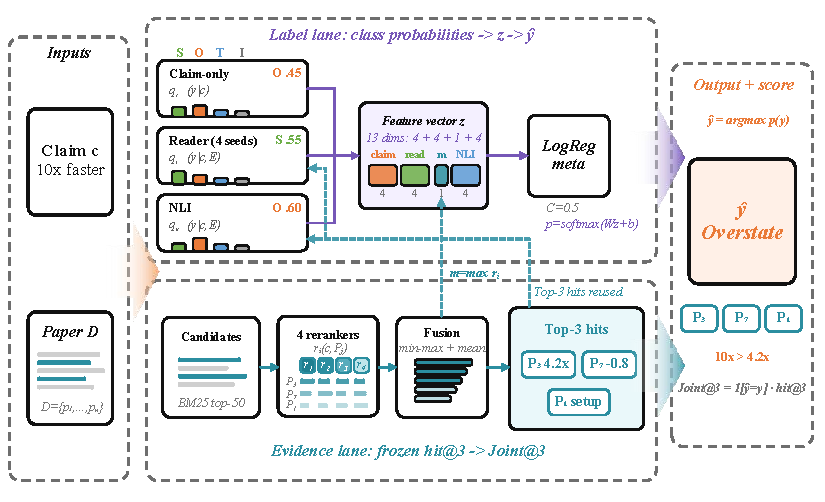
\includegraphics[width=\textwidth]{track2_figure.pdf}
\caption{Track~2 decoupled retrieval-and-labeling architecture. Fused rerankers select a fixed top-three evidence set, while reader, claim-only, and frozen NLI posteriors with the maximum fused score feed a logistic-regression meta-classifier.}
\label{fig:t2-system}
\end{figure}

The label module combines three complementary posterior estimates. The evidence reader models $p(y\mid c,E)$ from the claim and retrieved evidence, while the claim-only classifier estimates $p(y\mid c)$ and captures claim-side regularities that are less exposed to document-domain shift. The external multi-task NLI model treats the retrieved evidence as the premise and the claim as the hypothesis, yielding an entailment posterior without task-specific fine-tuning. Concatenating these probability vectors with the fused evidence score gives a stacked feature representation, which a logistic-regression meta-classifier~\cite{pedregosa2011sklearn} maps to the final citation-support label.

\section{Experiments}

\subsection{Track 1 Experimental Setup}
Track~1 uses the official train--development set and the Phase~1 test set. We split training data at the record level to prevent sentences from the same paragraph from appearing in different subsets. For offline evaluation, we also construct a development set with no shared image SHA values and reshape its minority-class density to approximate Phase~1. The official scorer reports sentence-level \mf{}, \pem{}, and their mean. Qwen3-VL-8B-Instruct serves as the backbone. LoRA is applied to all linear projections with rank 16 and $\alpha=32$, while the vision tower remains frozen. We train in bf16 with ms-swift 4.2.3 and set the image budget to \texttt{max\_pixels=401408}. Across 86 Codabench submissions under the official shared-task protocol, we compare single models, union ensembles, oversampling rates, softmin-PEM and plain-CE, image resolutions, an OCR channel, and suppression-based post-processing; the hidden Phase-2 test provides an unbiased estimate of the final system. Measured inference costs are reported in Appendix~A.

\subsection{Track 2 Experimental Setup}
Track~2 fine-tunes only on official task data; publicly available pre-trained models are used as frozen components without further tuning on non-official data, and inference uses no network access. The evidence module fuses BM25 candidates reranked by two DeBERTa-v3-large cross-encoders, MonoT5-large, and frozen Qwen3-Reranker-4B. The DeBERTa rerankers use a listwise grouped-softmax objective with hard negatives from the BM25 top-50 pool and differ by random seed and mining round. MonoT5-large is fine-tuned for three epochs with a learning rate of $3\times10^{-5}$.

The label module uses a DeBERTa-v3-large NLI reader, a claim-only classifier, and frozen tasksource-NLI. The reader uses a checkpoint trained on MNLI, FEVER-NLI, ANLI, LingNLI, and WANLI, and encodes the claim with the top three evidence paragraphs. It uses focal loss with $\gamma=2$ and inverse-frequency class weights. We train four seeds, 42, 13, 123, and 7777, for four epochs at learning rate $2\times10^{-5}$, batch size 8, gradient accumulation 2, warmup ratio 0.1, weight decay 0.01, and cosine scheduling, and average their probability vectors at inference. The claim-only classifier uses the same backbone and loss on claim text alone, with maximum length 256 and batch size 16.


\section{Results and Discussion}

\subsection{Track 1 Comparison and Sensitivity Analysis}
\label{sec:t1-sensitivity}
Table~\ref{tab:t1-leaderboard} reports the official Track~1 results for the five highest-ranked systems, including the final score and the scores for both phases. \method{}(\sys{}) ranks second with a final score of 68.7895, trailing the 68.8957 score of SUAT-NLP by 0.1062. Its Phase~2 score of 86.9652 is the highest among the five systems, indicating strong performance on the hidden phase. The remaining difference in the final score is mainly attributable to the 1.2320-point gap in Phase~1.

\begin{table}[H]
\centering
\caption{Official Track~1 results for the five highest-ranked systems. Submitter, organization, and member information is omitted.}
\label{tab:t1-leaderboard}
\small
\begin{tabular}{lccc}
\toprule
System & Final & Phase 1 & Phase 2\\
\midrule
SUAT-NLP & \best{68.8957} & \best{51.8457} & 85.9456\\
\method{}(\sys{}) & 68.7895 & 50.6137 & \best{86.9652}\\
BIT-TrustAI & 57.9880 & 44.0947 & 71.8814\\
ZZUNLP\_Han & 55.4690 & 42.4415 & 68.4965\\
YNU-HPCC & 46.1610 & 31.9323 & 60.3898\\
\bottomrule
\end{tabular}
\end{table}

Table~\ref{tab:t1-results} shows how the Phase~1 score varies with minority prediction density, ensemble size, and the training recipe. Increasing the number of minority predictions from 46 for the near-all-\lab{Supported} baseline to 253 for the best single model raises the score from 18.85 to 47.80. This result identifies minority-class recall, rather than minority-class suppression, as the main bottleneck on the test set. Increasing the union from one to five members further raises the score from 47.80 to 50.26, and the final density-augmented union reaches 50.61. The loss comparison depends on the data recipe. Under controlled data conditions, plain-CE outperforms softmin-PEM both without oversampling, 38.68 versus 34.21, and on the same oversampled data, 42.87 versus 39.14. The best single model scores 47.80 with softmin-PEM, but it uses more aggressive \lab{Supported} downsampling than the plain-CE configuration. The effects of the objective and data recipe are therefore not fully separated in this comparison.

\begin{table}[H]
\centering
\caption{Track~1 sensitivity analysis. Score is the official Phase~1 score, and \#Min. is the number of minority-class predictions. The final recipe marked by $^{\dagger}$ uses stronger \lab{Supported} downsampling and is not a controlled comparison with the plain-CE row.}
\label{tab:t1-results}
\small
\begin{tabular}{llrr}
\toprule
Factor & Setting & Score & \#Min.\\
\midrule
\multirow{5}{*}{Minority density} & Near-all \lab{Supported} & 18.85 & 46\\
& suppression-1 & 38.48 & 127\\
& suppression-2 & 39.57 & 171\\
& union of three & 43.85 & 190\\
& best single & 47.80 & 253\\
\midrule
\multirow{5}{*}{Union size} & 1 member & 47.80 & 253\\
& 3 members & 48.22 & 339\\
& 4 members & 49.99 & 365\\
& 5 members & 50.26 & 382\\
& final union & \best{50.61} & 399\\
\midrule
\multirow{5}{*}{Loss / sampling} & softmin, no oversampling & 34.21 & --\\
& plain-CE, no oversampling & 38.68 & --\\
& plain-CE, oversampling & 42.87 & 245\\
& softmin, oversampling (same data) & 39.14 & --\\
& softmin, oversampling (final recipe)$^{\dagger}$ & 47.80 & 253\\
\bottomrule
\end{tabular}
\end{table}

\subsection{Track 2 Results}
Tables~\ref{tab:t2-final} and~\ref{tab:t2-ablation} report the final Track~2 leaderboard and label-side ablation. \method{} ranks first among 15 teams with a final score of 86.27, exceeding the second-ranked system by 3.28 points. It scores 86.21 in Phase~1 and 86.33 in the blind Phase~2 evaluation, a difference of only 0.12. Its \joint{} score of 81.37 exceeds that of the second-ranked system by 4.94 points and accounts for most of the final margin.

\begin{table}[H]
\centering
\caption{Five highest-ranked Track~2 systems and the official prompting
baselines. The final score is the mean over both phases; \mf{} and \joint{}
are two-phase aggregates, while baseline rows report Phase~1 values.}
\label{tab:t2-final}
\small
\begin{tabular}{clccccc}
\toprule
Rank & Team & Final & \mf{} & \joint{} & Phase~1 & Phase~2\\
\midrule
1 & \method{}(\sys{}) & \best{86.27} & 91.18 & \best{81.37} & \best{86.21} & \best{86.33}\\
2 & Lenormand System & 82.99 & 89.55 & 76.43 & 81.28 & 84.70\\
3 & HER-DAC & 81.61 & 93.05 & 70.16 & 81.70 & 81.52\\
4 & ZZUNLP\_Han & 81.38 & \best{94.25} & 68.51 & 80.88 & 81.88\\
5 & SUAT-NLP & 79.01 & 91.02 & 67.00 & 80.88 & 77.13\\
\midrule
-- & GPT-5.4 (prompting) & -- & 41.65 & 39.38 & 40.51 & --\\
-- & Gemini 3.1 Pro (prompting) & -- & 46.02 & 31.91 & 38.97 & --\\
-- & Qwen3.6-Plus (prompting) & -- & 38.08 & 22.63 & 30.35 & --\\
\bottomrule
\end{tabular}
\end{table}

\begin{table}[H]
\centering
\caption{Label-side ablation on Track~2 Phase~1. All three systems use identical evidence lists.}
\label{tab:t2-ablation}
\small
\begin{tabular}{lccc}
\toprule
Label system & Track~2 score & \mf{} & \joint{}\\
\midrule
Four-seed reader (baseline) & 83.10 & 87.02 & 79.19\\
$+$ claim-only mixture ($w=0.8$) & 85.10 & 89.41 & 80.79\\
$+$ NLI feature and meta-classifier & \best{86.21} & \best{90.46} & \best{81.96}\\
\bottomrule
\end{tabular}
\end{table}

With the evidence list fixed, the claim-only mixture adds 2.00 points, and the NLI feature with the meta-classifier adds a further 1.11 points. Both changes improve \mf{} and \joint{} because they correct labels for records whose evidence has already been retrieved. By contrast, changing the evidence-fusion function, adding a fifth reranker, or attempting to exploit the third evidence slot provides no gain. Two teams achieve higher final \mf{} scores than ours but lower overall scores because their \joint{} values are 11.2 and 12.9 points lower. The official metric therefore rewards a balance between retrieval and label prediction rather than a stronger reader alone.

\subsection{Negative Results and Transferable Lessons}
Both tracks produce informative negative results. In Track~1, higher image resolution, two-epoch training, supervised chain-of-thought, OCR, and weak or incorrectly correlated heterogeneous members do not give consistent gains, leaving minority-recall union as the transferable strategy. In Track~2, zero-shot and few-shot frontier LLM annotation reaches only 58.9--64.4\% development label accuracy, far below the 95.9\% of the fine-tuned reader. Domain-adaptive pretraining, domain-adversarial training, BBSE label-shift correction, SciNLI curriculum transfer, additional NLI features, and an eight-seed reader also fail selection. These failures show that stronger components do not automatically yield stronger shared-task systems: Track~1 models still miss dense minority-class sentences if they inherit the training prior, and Track~2 readers remain vulnerable when they directly read out-of-domain evidence. Effective designs instead exploit metric and distribution structure, namely recall additivity for Track~1 and label correction after frozen evidence for Track~2.

\section{Conclusion}

This paper presents \method{} for two-track scientific-report faithfulness verification. Track~1 uses Qwen3-VL-8B with LoRA, long-tail resampling, density-matched augmentation, and a recall-additive union for figure and table evidence, scoring 50.61 in Phase~1 with the highest \mf{} of 57.54 and ranking second overall with 68.79, 0.11 behind first place. Track~2 freezes four-reranker evidence fusion and stacks a DeBERTa reader, a claim-only signal, an external NLI posterior, and a logistic-regression meta-classifier for citation evidence, ranking first among 15 teams with 86.27. The results show that modality, distribution, and metric coupling shape performance: Track~1 is limited by minority recall and paragraph exact match, and Track~2 by retrieval-label coupling under domain shift. Limitations include partial reconstruction of the best Track~1 recipe, \pem{} nondeterminism, claim-only stylistic dependence, and a 433-record development set; future work should improve validation, evidence alignment, and transfer to human-written claims.

\appendix
\section{Supplementary Analysis for Track~1}
\label{app:t1}

\subsection{Inference Cost}
Table~\ref{tab:t1-cost} reports measured Phase-1 inference times (586 records, 5{,}096 sentences) on a single H100 with bf16 at the standard image budget, for the per-sentence Qwen3-VL-8B members of the union. The five-member union runs members in parallel, so its wall-clock time is bounded by the slowest member when GPU capacity is available.

\begin{table}[H]
\centering
\caption{Measured inference time on the Phase-1 test set (single H100, bf16, \texttt{max\_pixels=401408}).}
\label{tab:t1-cost}
\small
\begin{tabular}{lrr}
\toprule
Member & Minority predictions & Time\\
\midrule
Grid (s01) & 253 & 1{,}342\,s\\
Oversampling-4 (s08) & 236 & 1{,}177\,s\\
Per-class (s09) & 268 & 1{,}150\,s\\
\midrule
Union (5 members, parallel) & 382 & $\leq$~1{,}342\,s wall clock\\
\bottomrule
\end{tabular}
\end{table}

\FloatBarrier

\subsubsection*{Acknowledgments}
This work was funded by the Xinjiang Talent Development Fund (Grant No. XJRC-2025-KJ-PY-KJLJ-051).

\bibliographystyle{splncs04}
\bibliography{references}

\end{document}
